% Copyright (c) 2014,2016 Casper Ti. Vector
% Public domain.

\chapter{相关研究综述}
\section{地形高程表达}
地形在数学上可以表示为一个高程函数$h:\Omega\to\mathbb{R}$,$\Omega$表示XY平面上的一个连续的域,$\Omega \subset \mathbb{R}^2$。 $h$至少是$C^0$连续的函数,可以表示出$\Omega$中任意一点的高度。地形的表达有多种方法,分别在时间效率、空间开销等方面有所侧重。
\paragraph{函数表达}地形高程可以用一个闭式表达式作为函数$h$,并在实际应用时将函数采样为一个有限的点集,作为地形数据\supercite{CignoniRepresentation}。这种表达方式在内存上非常紧凑,且表达精度没有限制,但获取给定点$p$的高程$h(p)$时需要计算得出。理论上任何合适的函数$h$都可以用来表示高程,但构造一个能真实反映地形地貌特征的函数是一项复杂的任务。
\begin{figure}[htbp]
\centering
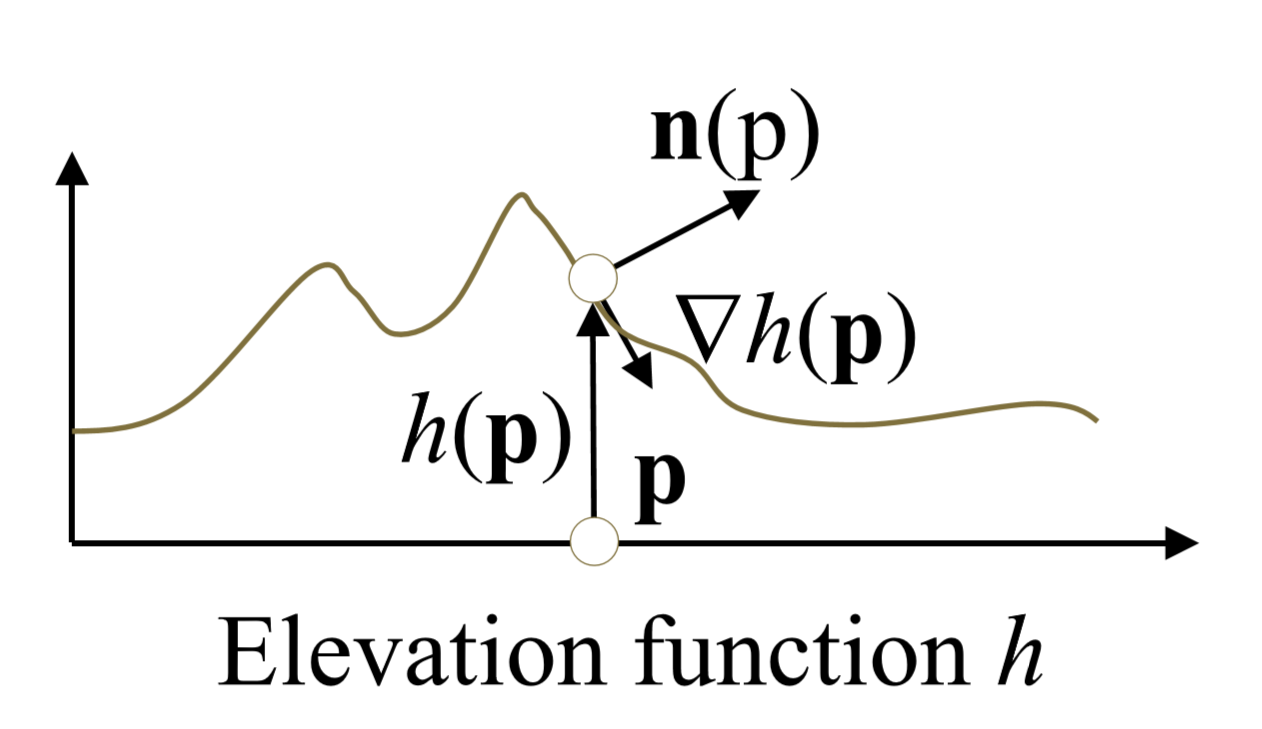
\includegraphics[height=4cm,width=6.9cm]{figures/continue.PNG}
\caption{以函数形式表达高程\supercite{eric-review}}
\end{figure}
\paragraph{离散高度场表达}地形高程也可以由一组排列在规则2D网格上的离散高程值表达,并可以以灰度图的形式存储,称为高度图。这种表达方法不能模拟悬垂和洞穴等特征,但由于其能简单和有效利用存储空间,因此是工业界目前最常用的地形表达方式,被广泛应用于GIS应用、地形编辑工具、地形腐蚀模拟和游戏等领域。高度场数据通常由遥感卫星捕获得到,其精度受到网格大小和网格内部点个数的影响。要获得连续的表面数据需要在格点之间进行插值,通常的做法是对单元内的两个三角形进行两次线性插值。与函数表达不同,这种表达可以更好的支持不同形式的地形,但和过程式表达相比增加了内存开销。一种减小内存开销的方法是降低数据精度,用8位或16位表示一个数据。
\begin{figure}[htbp]
\centering
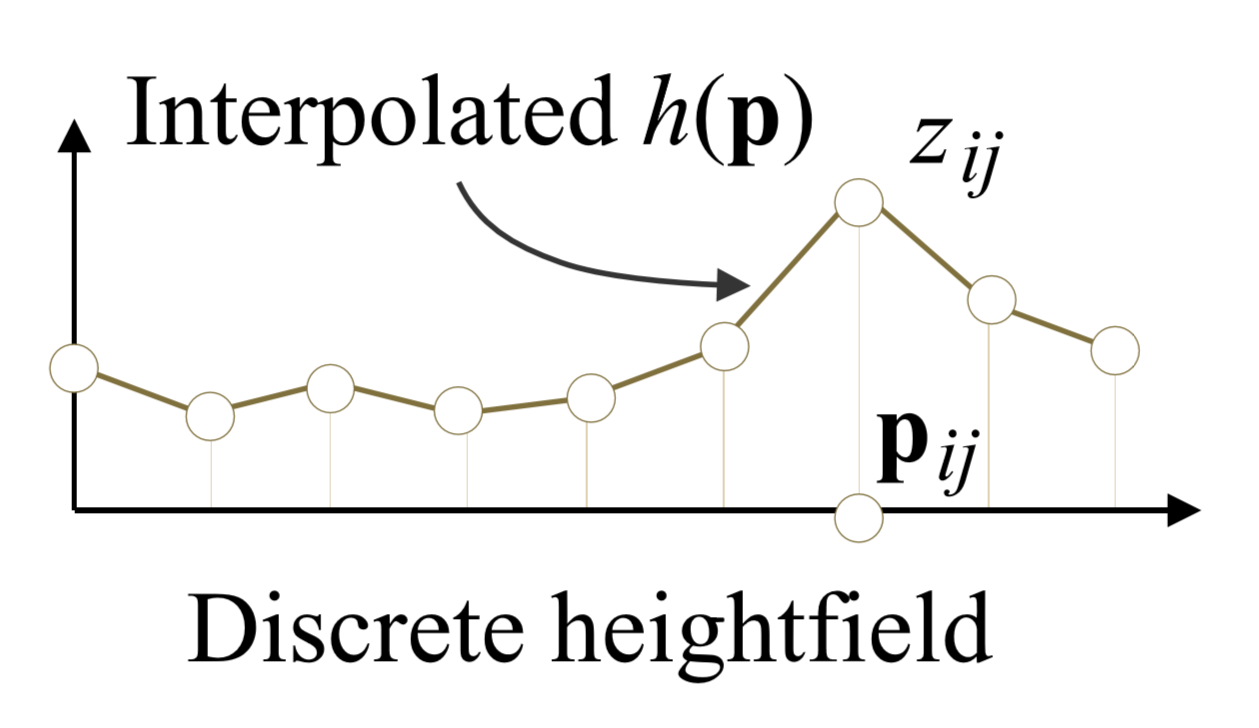
\includegraphics[height=4cm,width=6.8cm]{figures/discrete.PNG}
\caption{以离散数据形式表达高程\supercite{eric-review}}
\end{figure}
大规模地形通常分块存储数据,以减少数据调度给内存带来的压力。网格数为$n$的块在每个网格格点上保存一个高程值,总共保存$(n+1)*(n+1)$个数据。为使地形块之间正确的拼接,对于索引为$(x,y)$的瓦块,其右边界与其右边块$(x+1,y)$的左边界相重叠,同理,其下边界与其下边块$(x,y-1)$的上边界重合。

\paragraph{体素表达}
体素表达可以捕获不同地质层的褶皱和断层,从而允许有悬崖、洞穴和拱桥的地形,解决了高度场表达不能反映地形的内部结构的问题。在这种方法中,空间被划分为3D规则网格,每个单元分配一个材质索引。由于进行了显式空间枚举,这种表达方法内存开销非常高,可以通过稀疏体素八叉树等技术进行压缩优化。此外,其离散特质使其不适合进行高精度的平滑地形建模,如非常平缓的斜坡等。\par
体素表达模型可以由一个函数定义$\mu:\mathbb{R}^3\to \digamma$,其中 $\digamma\subset\mathbb{N}$表示空间中任意体素所使用材质的索引。可以用单一材质的模型表示不具备语义信息的地形,即$\digamma=\left\{0,1\right\}$,其中0为空气,1为基岩。对于含有语义信息的地形,可以扩展索引集,使体素的材质索引表达语义信息,如图2.2。
\begin{figure}[htbp]
\centering
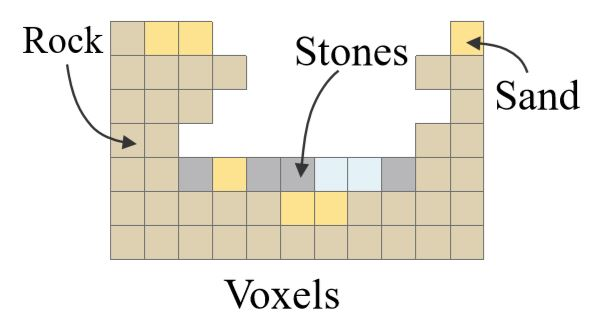
\includegraphics[height=3.8cm,width=7cm]{figures/voxel.JPG}
\caption{体素表现允许拱桥、洞穴或悬崖的建模,但形状受其离散性的限制。\supercite{eric-review}}
\end{figure}

\paragraph{分层表达}
分层表达通过对地表不同沉积物的厚度进行建模来表达地形。Musgrave等\supercite{Musgrave1998The}提出了材质层的概念,并将不同材质层编码为一组有序的函数,这些函数在预先建立的层中描述厚度。其中底层表示基岩的高程,后续每一层表示其他物质的厚度,如岩石、沙砾、水等。这种数据结构是高度场表达法和体素表达法在空间效率上的折中,将体素表达法的数据压缩为了高度场的堆栈。此外分层表达法的垂直分辨率可以是无限的,而体素是离散数据,因此比起体素表达法,分层表达法可以更好的表达拱桥、悬崖等地形。以不同材质的复杂的动态堆栈管理为代价,分层表达法在地形腐蚀模拟中也得到了广泛的应用。
\begin{figure}[h]
\centering
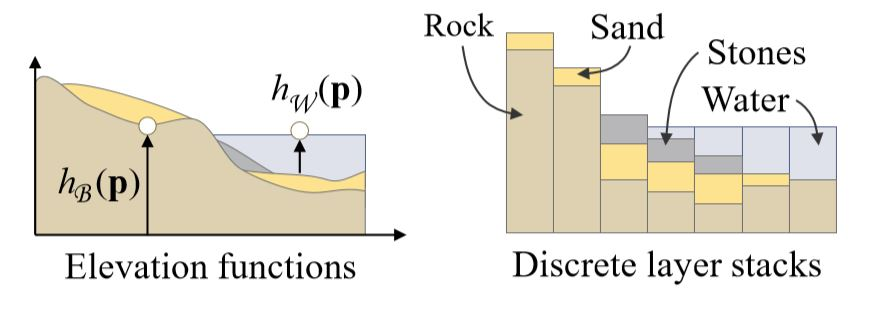
\includegraphics[height=4cm,width=11.5cm]{figures/layer.JPG}
\caption{分层模型表达了按照预先设定的顺序组织的不同材质(从底向上依次是基岩、沙子、岩石和水)\supercite{eric-review}}
\end{figure}

\section{大规模地形实时渲染}
大规模地形数据的规模远远超过了标准图形硬件的能力,如果没有很好的地形表达和渲染算法的支持,就不可能以高细节层级交互式的进行可视化。在大规模地形实时绘制中,地形数据往往组织成四叉树形式。\supercite{Pajarola1998Large}
\subsection{地形四叉树}
地形四叉树是目前组织大规模地形的常用解决方案,它以分层的形式存储多分辨率地形数据,并将整个地形数据划分为若干个规则网格,每个网格被称为一个地形块。地形块在概念上被安排在不同的层次上,每个块上一层次的数据都被降采样到其一半的分辨率,类似于纹理数据的Mipmapping概念。如图2.5所示,每一层的网格被细分为许多大小相等的正方形块,每个块包含固定数量的高度值,块中的数据都是连续存储的。\par
\begin{figure}[H]
    \centering
    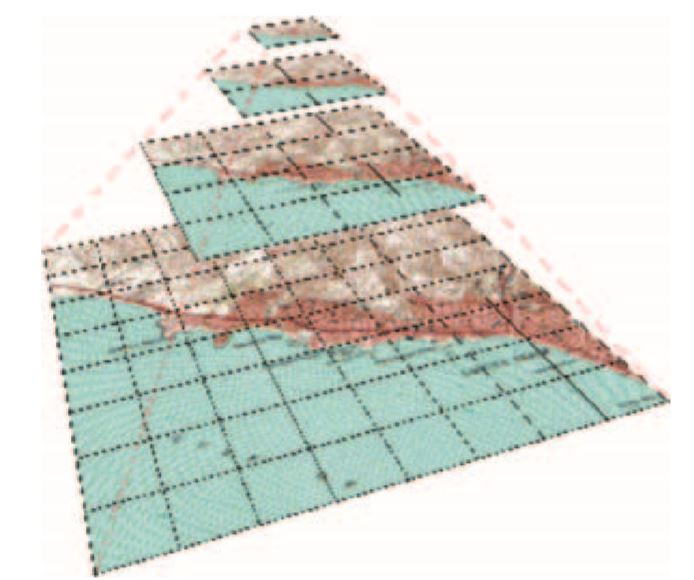
\includegraphics[height=4cm,width=4.8cm]{figures/quadtree.jpg}
    \caption{存储为瓦块金字塔的地形\supercite{PlatingsCompression}}
\end{figure}
完整的四叉树存储意味着一个节点和它的子节点和邻居节点之间存在简单的位置关系,确定最顶层的经纬度范围和子块的大小后,各个级别之间的关系就被确定了,无需存储指针,可以直接从块索引中得到一个节点的位置关系。\par

地形四叉树根据视点位置来请求子节点,使CPU资源可以集中服务关键部分的数据。以不同层级渲染的地形块由于分辨率不同,可能会在地形块接缝处产生裂缝(图2.6),这种缝隙被称为T形连接(T-junction)。如图2.7所示,消除T形连接引起的裂缝有两种方法,第一种方法是将高分辨率网格中的边界点值与低分辨率点对齐。第二种是在低分辨率块中插入新点,并将值设置为高分辨率块中的对应点。第一种方法更加快速,但在网格边界高程变化剧烈的地形块上,减少三角形会降低画面质量,因此第二种方法视觉效果更好。
\begin{figure}[H]
    \centering
    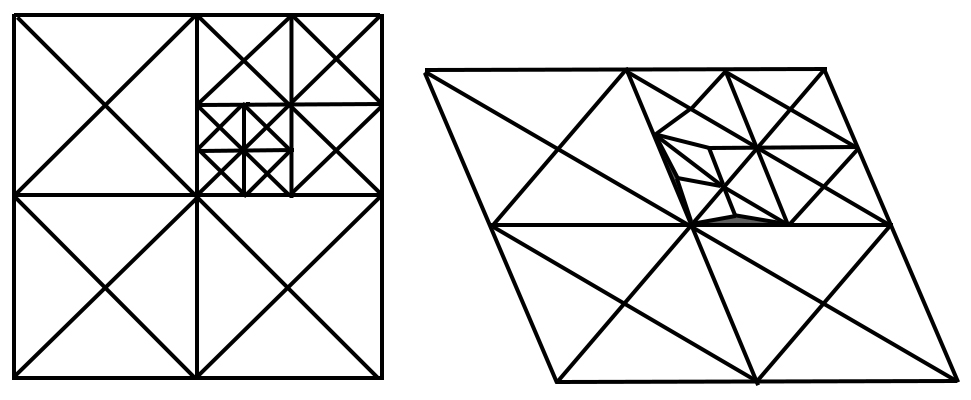
\includegraphics[height=3.5cm,width=9.2cm]{figures/seam2.jpg}
    \caption{四叉树的三角剖分及产生的裂缝。左图中的黑点处可能产生裂缝,右图中的阴影部分显示了这些裂缝。\supercite{You2003Real}}
\end{figure}
\begin{figure}[H]
    \centering
    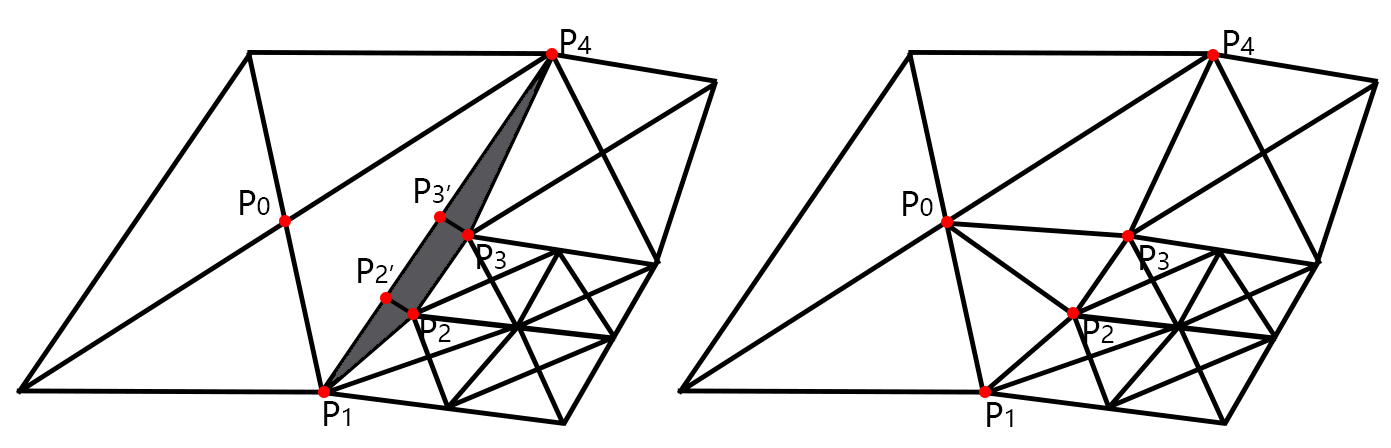
\includegraphics[height=3.7cm,width=10.2cm]{figures/seamRepair.png}
    \caption{消除裂缝的两种方法。左图显示了第一种方法,将点$P_2$,$P_3$拉至点${P_2}^{'}$,${P_3}^{'}$处;右图显示了第二种方法,在低分辨率块中增加点,并与高分辨率块缝合\supercite{You2003Real}}
\end{figure}
\subsection{地形实时渲染技术}
大规模地形渲染的主要挑战是保证渲染效率的同时,兼顾地形的规模和精细程度。通过在CPU端对地形数据集的大小进行优化、在GPU端增添视觉增强策略等方法,可以提升地形的渲染效率和精细程度。下面介绍了实时渲染中一些实用的技术。
\paragraph{视锥剪裁}
为了最大限度地减少每帧渲染三角形的数量,需要对等待绘制的地形块进行视锥剪裁,将不在视锥中的块及其子块排除在外,使渲染性能显著提高。将地形块的包围盒与视锥体进行求交测试,与视锥相交的地形块被绘制,完全没有交集的地形块被直接抛弃,其数据不会被传输给GPU。在四叉树的数据结构中,如一个地形块的测试结果为不可见,则其子块也不可见。这个特性使剪裁算法可以非常快速的执行,减少了CPU的工作量。同时如果一个地形块完全位于视锥体内,则其子块也完全位于视锥体中,无需再进行测试。\par
视锥中的物体不一定都可见,也可能被其他物体遮挡而导致不可见。对于绘制地球的应用,地球自身遮挡其背面的地形,位于观察视角地平线下的地形块是无需绘制的,因此还可以进行遮挡剪裁来提升效率。

\paragraph{数据请求预测}
稳定的帧率对于仿真类应用有重要的意义。在对大规模地形场景进行渲染时,假设有三个连续的场景,渲染时以三个连续的视窗体现,分别是$w_1$、$w_2$和$w_3$。为了实现块数据缓冲,当发送$w_1$的块请求时,同时发送$w_2$和$w_3$的块请求。三个窗口的块请求的优先级不同,在$w_1$中的块请求应该被设置为优先,而$w_2$的块请求中,除去与$w_1$公有的部分,其他部分应该设置为次优先,在$w_3$的块请求中,除去其与$w_1$和$w_2$公共的部分,应该设置为低优先级,如图2.8所示。因此,当场景移动到$w_2$时,系统发送$w_2$窗口的块请求,数据预测线程将直接从地形渲染涉及的缓冲区中获取数据,而不需要从磁盘中读取数据。可以根据每秒画面刷新的次数和在场景中的移动速度决定预测请求的半径。使用类似的技术,在固定路线的场景漫游或飞行视景仿真中可以提高画面帧率的稳定性。\supercite{Chen2010Design}
\begin{figure}[htbp]
\centering
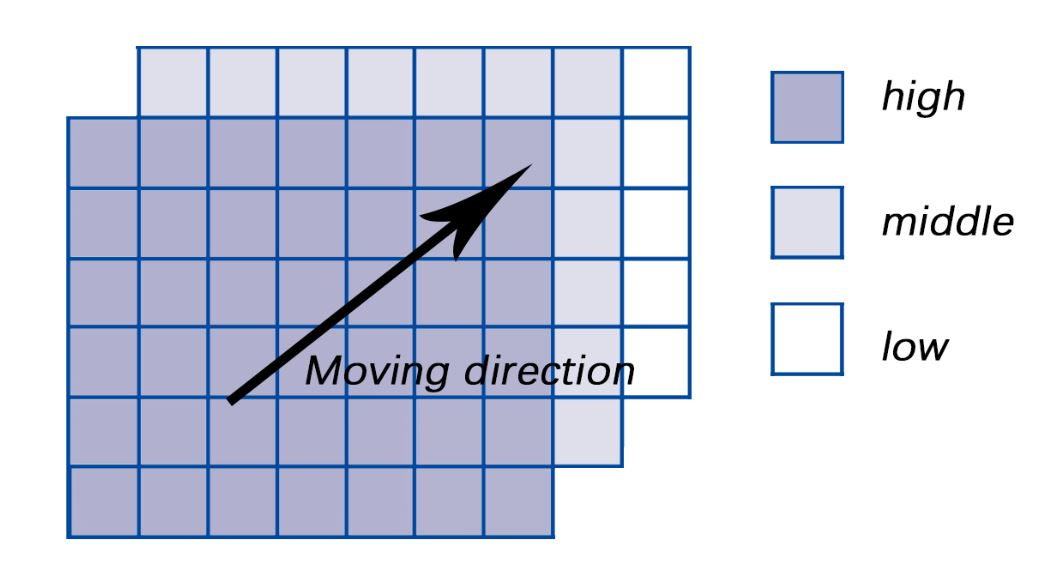
\includegraphics[height=4.3cm,width=7.8cm]{figures/predic.JPG}
\caption{预测的数据块按高中低三个优先级进行顺序请求}
\end{figure}

\paragraph{过程式渲染}
过程式生成技术和硬件曲面细分技术允许在使用低分辨率的数据集情况下,仍然提供非常精细的地形可视化,而无需很高的存储开销。在游戏等许多应用中,地形数据高度值的准确性不是很重要,可以采用分形压缩算法将地形压缩成小而紧凑的数据集,并在运行时构建高精度的地形,从而大大减小地形数据的大小。为了动态的增强粗糙网格场景的细节,一个解决方案是在粗网格靠近相机的时候,通过程序过程式的细化粗网格或纹理。基于CPU的网格细化会被庞大的CPU-GPU几何数据流式传输所阻塞,为了避免这些数据传输,大量工作致力于通过利用曲面细分着色器直接在GPU上实现或模拟这些递归细分算法。Dachsbacher等\supercite{Dachsbacher2004Rendering}描述了一种动态向地形添加细节的方法,用数字高程图定义地形的大致形状,在渲染过程中,在图形硬件添加过程式的高程和纹理细节。Gu等\supercite{GuGeometry}将由草图生成的粗糙地形高度存储在几何图像中,并在绘制阶段加入详细的分形噪声。\par

\paragraph{贴花技术}
贴花是一种游戏开发中常用的贴图技术,其主要思想是在物体表面附加一张贴图,以实时的实现弹孔,血液喷溅痕迹,墙面涂鸦,脚印等等效果。此类技术有很多种表现形式,可以在物体表面附加半透明贴图、分层材质甚至模型。地形生成领域也可以将贴花技术用于为现有地表纹理添加高频率、高分辨率的细节,以极低的成本大大增加近地表漫游时的真实感。如在田野或机场的草地上添加草叶状图案、或在跑道和道路上添加砾石图案。贴花技术可以最小化顶点数,可以依据对渲染效果和效率的需求,轻松地调整低分辨率网格的LOD,且开销极低。因此,尽管在制作流程上需要一些额外的处理,但贴花技术有时可以作为地形曲面细分技术的替代方案。

\section{地形生成技术}
\paragraph{基于分形噪声的生成}
基于分形噪声的地形生成方法是一种过程式技术,此方法不模拟塑造地形的物理过程且不使用真实数据作为范例,而是通过对现实世界的观测直接重现现象。在观测中,真实地形常常表现出具有分形特征的分枝结构或树状图案,分形噪声可以很好的模拟出地形在多个尺度上的自相似性。分形噪声是早期的地形生成中最常用的过程模型之一,具有实现简单、效果良好、占用资源少等特性。\par
用分形噪声生成地形是在$\mathbb{R}^2$上定义一组经过缩放和变形的噪声函数\supercite{fbm},通过添加不同尺度和振幅的噪声,构建一个表示真实地形的函数。设$n$表示从$\mathbb{R}^2$到$[−1,1]$区间映射的平滑噪声函数,湍流函数$t$的定义是将不同频率和振幅的噪声贡献相加:
\begin{equation}
t(p)=\sum_{i=0}^{k-1}a_in(\Phi_ip)
\end{equation}
其中,$a_i$表示不同的振幅,$\Phi_i$表示不同频率,$k$表示噪声函数的个数。一般来说,振幅和频率被定义为一个几何级数:
\begin{equation}
\begin{aligned}
a_i=a_0p^i \\
\Phi_i=\Phi_0l^i
\end{aligned}
\end{equation}
其中$a_0$和$\Phi_0$是基础振幅和频率,$p$和$l$分别表示振幅的减益和频率的增益,在地形生成中通常将$p$设置为0.5可以得到有良好局部性和丰富细节的地形。噪声函数$n$的平滑性可以防止在山地地形中创建峰和脊线,如图2.9左图所示。因此为了产生诸如山峰或脊线之类的尖锐特征,可以引入脊线噪声。脊线噪声可以简单地定义为$r(p) = 1-|n(p)|$,其效果见图2.9右图。
\begin{figure}[htbp]
\centering
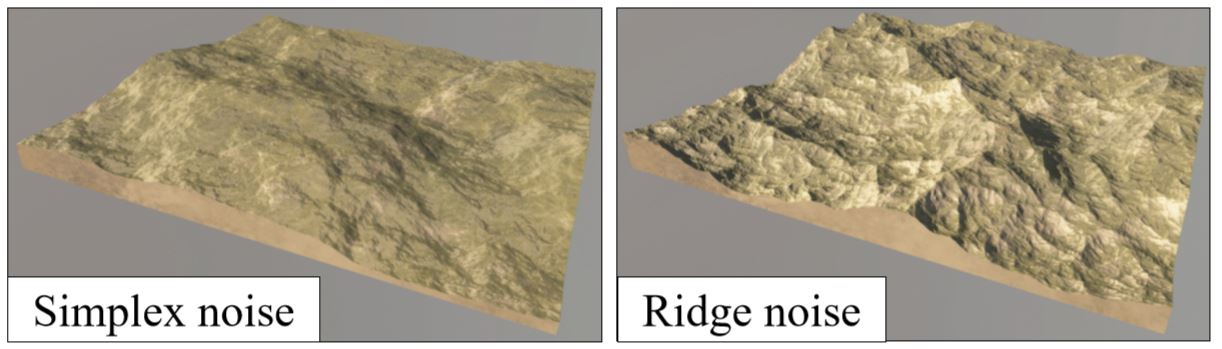
\includegraphics[height=3.5cm,width=11.4cm]{figures/fractal.JPG}
\caption{分形噪声生成的过程式地形,左图为平滑噪声生成的地形,右图为八个不同频率的脊噪声叠加形成的多重分形地形\supercite{eric-review}}
\end{figure}
\paragraph{基于草图的生成}
基于草图的方法也称为基于特征的方法,该方法接受用户输入生成特征曲线,如山脊线,海岸线或河流等,并通过特征线将地形特征扩散至整个地形,从而生成匹配这些地形特征,且宏观上具有一致性的地形。Gain等\supercite{gain-sketching}的工作代表了最早的基于草图的方法之一,用于从控制曲线对地形进行交互建模。用户通过各种速写曲线来指定地形,可以输入的信息包括:基线(表示山脊在地面上的投影)、海拔(捕捉山脊的垂直形状)和边界(限制地形延伸到基线两边的距离)(图2.10)。\par
\begin{figure}[htbp]
\centering
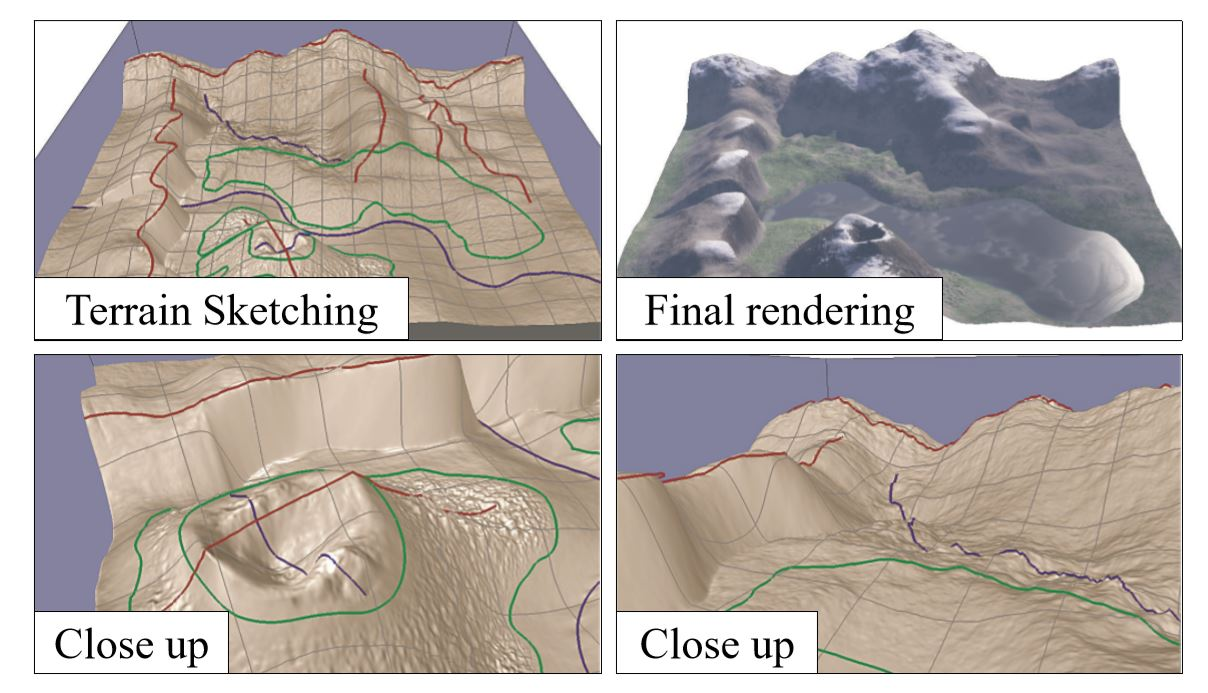
\includegraphics[height=5.6cm,width=9.9cm]{figures/sketching.JPG}
\caption{草图可以将山峰、悬崖、火山锥、不同方向的小山和河流峡谷都在一个单一的地形中被描绘出来\supercite{gain-sketching}}
\end{figure}
Hnaidi等\supercite{HnaidiFeature}用特征曲线表示出山峰、河流和主要河流地貌的骨架,从而创建出地形。其使用带有附加信息的二维样条作为特征曲线,并描述了曲线每一侧的高程和坡度信息。由此产生的基于矢量的模型在内存中非常紧凑。噪声参数和梯度约束通过一个标准的扩散方程在离散网格中传播,对地形表面进行重构。通过使用扩散噪声参数合成的噪声图生成细节,向平滑的扩散地形添加细节来获得最终的地形。\par
基于特征的生成方法的提供了一种更直观的用户控制,但主要挑战来自于在整个地形上传播稀疏信息的困难,例如,在整个地形上传播山峰或河流等特定的地形信息。
\paragraph{基于仿真的生成}
过程式方法着重于一个特定现象的产生,而仿真技术注重模拟现象产生的原因和结果,因此能产生更真实的结果。地形仿真可以被看作是一个复杂的系统,在这个系统中,各种影响地形的元素相互作用产生了特殊的地貌。大部分的使用仿真技术的地形生成算法都是基于侵蚀的。侵蚀可以被抽象为一个三步过程,物质被侵蚀并从底层地形中分离出来,然后被介质运输,最终沉积在不同的位置(如图2.11)。侵蚀过程包括但不限于降雨和地表径流、河流和小溪侵蚀、海岸和海洋侵蚀、冰川侵蚀、风力侵蚀和大规模运动。\par
\begin{figure}[htbp]
\centering
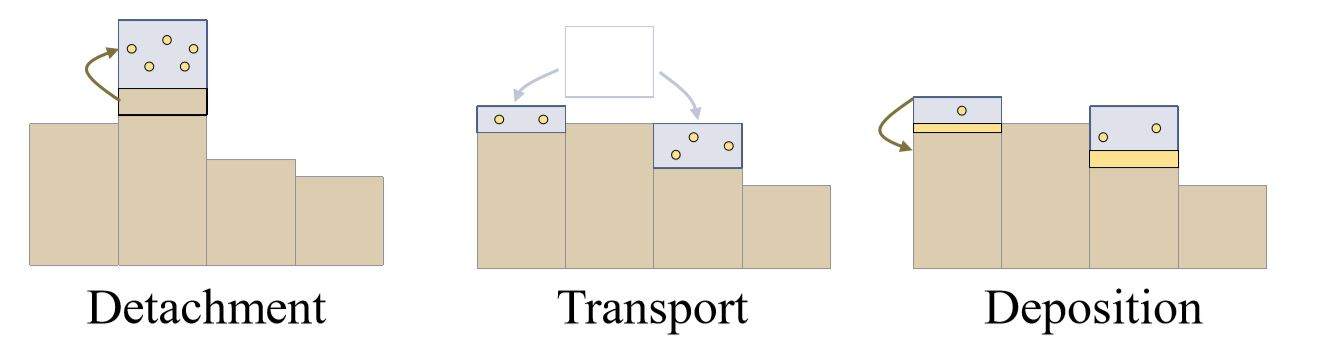
\includegraphics[height=3.6cm,width=12.5cm]{figures/simulation.JPG}
\caption{侵蚀过程分离一些物质,由介质运输物质,最终沉积在不同的位置\supercite{eric-review}}
\end{figure}
Musgrave等\supercite{Musgrave1998T}在其工作中介绍了基于热力学的地形侵蚀方法。热侵蚀是热风化和物质运动相结合的产物,由于温度的变化,存在于物质缝隙中的水和物质本身产生了不同的热膨胀,引起物质的破裂,并在重力作用下向下运动。由此产生了宏观视角上,斜坡上的岩石和沉积物向下运动的现象。
\begin{figure}[htbp]
\centering
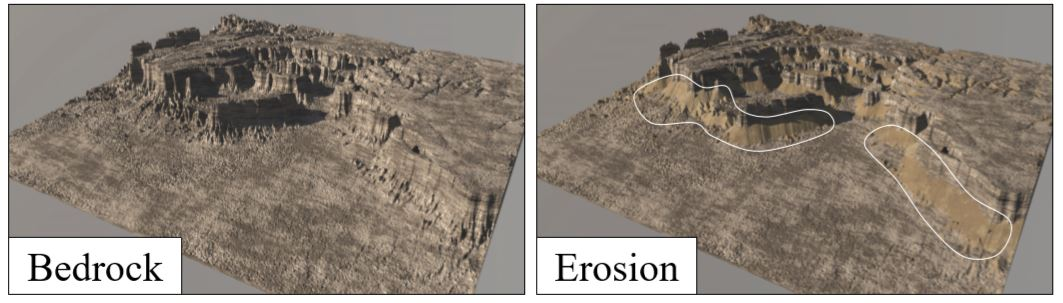
\includegraphics[height=3.5cm,width=11.4cm]{figures/thermal.JPG}
\caption{热力侵蚀:左图是裸露的基岩,右图是热侵蚀形成的山岩和悬崖底部的岩屑和碎石\supercite{eric-review}}
\end{figure}
Benes等\supercite{Bene2002Visual}提出了一种水力侵蚀算法,算法通过一个离散的基于网格的模型来表示输入场景和流体,模拟水压力、水流速度和每个网格中的流体量。该水力模拟模型可以模拟水溶解土壤,转移土壤,并通过重力沉降将其沉积在不同的位置的过程。水力侵蚀可以在高峰之间形成深沟,而热力侵蚀可以正确地在岩石层创造岩石、沙子和颗粒物质,可以作为水力侵蚀的一个重要补充步骤。
\begin{figure}[htbp]
\centering
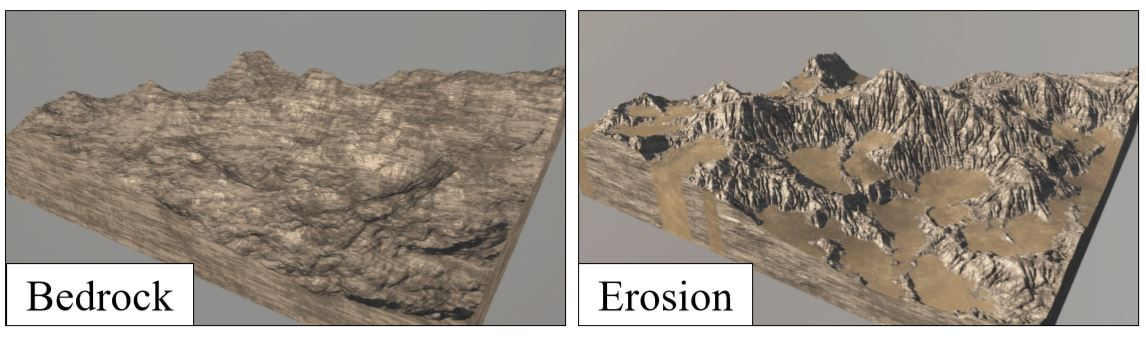
\includegraphics[height=3.5cm,width=11.4cm]{figures/hydraulic.JPG}
\caption{水力侵蚀应用在过程式地形上的效果\supercite{eric-review}}
\end{figure}
\paragraph{基于样例的生成}
基于样例的方法借鉴并结合现有的地形,通过过程式方法或仿真方法逐步构建地形。样例地形的数据可以有多种来源,最常用的是来自于遥感卫星采样得到的真实数据,但也可以来自于过程式和仿真方法输出的地形。典型的基于样例的地形生成管线如下:(1)构建包含一个或多个地形样例的数据库;(2)执行分析步骤,从数据库中选择、扭曲和排列地形片段,并获取其高程函数;(3)将多个片段融合在一起,输出一个无缝的地形。基于样例的方法常常使用地形高程图作为算法的输入输出。Zhou等\supercite{Zhou2007Terrain}提出了一个基于纹理生成地形高度图的方法,该高度图受到用户输入的曲线特征的约束。给定一个用户绘制的草图和一个作为风格输入的真实地形,算法通过从真实地形复制像素块来创建一个新地形,这样用户草图中指定的曲线特征会呈现在输出中,且生成的真实地形具有与真实地形相同的小尺度特征。但是泊松接缝去除技术(一种去除重叠的块产生的人工痕迹的块合并技术)在3D光照下会产生明显的人工痕迹。此外用户只能指定山谷和山脊线的位置,2D草图不允许对这些特征线的高度轮廓进行直观的控制。Tasse\supercite{TasseEnhanced}等对这种技术进行了扩展,通过GPU并行计算降低了选取最佳块的成本,并减轻了多个块重叠造成的不自然痕迹。\par
\begin{figure}[htbp]
\centering
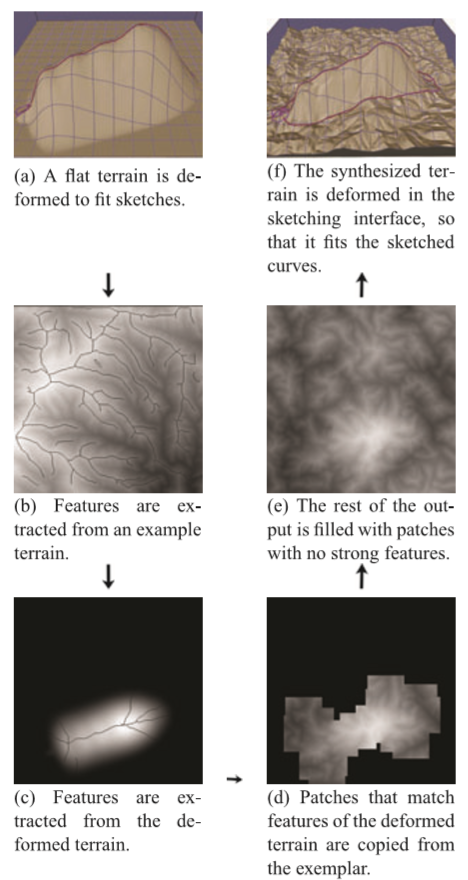
\includegraphics[height=11cm,width=6cm]{figures/patchBased.PNG}
\caption{基于样例生成地形的工作框架\supercite{TasseEnhanced}}
\end{figure}
虽然这种方法快速、可控且生成的地形非常真实,但此类基于数据的方法需要上游训练阶段,且其结果高度依赖于输入数据的质量,采样的分辨率也局限于样例的分辨率,而公共可用的地形数据资源通常在每像素几米的范围内。

\section{地形生成结果评价标准}
对于给定的地形生成方法,有几个判断其有效性和实用性的标准。不同的应用场景依照其对各项标准的侧重,选择适合的地形生成算法。\supercite{eric-review}
\paragraph{多样性}
地球上有各种各样的地形,包括山丘、山脉、高原、峡谷和山谷等等。它们可能是由主要的自然事件或现象造成的,也可能是由许多不同因素在很长一段时间内的复杂相互作用造成的。地形可根据其高程、方向、坡度、土壤类型、基岩暴露状况等特征进行分类,地形生成算法能否产生多种多样的地形是评价标准之一。
\paragraph{真实感}
目前的地形生成方法中,在真实感方面普遍存在两个问题:(1)无法在不同尺度上都得到精确丰富的细节;(2)地形生成算法通常只能对一种现象进行模拟,难以将不同生成过程产生的地貌结合在一个地形中。评估地形真实感的一种方法是用地形渲染图对观察者进行用户调研,另一种方法是使用模拟水流对生成的地形进行排水的一致性测试。感性的和定量的评价方法不一定能得出一致的结论,因为某些现实世界的地貌,对从未见过此类地貌的观看者来说可能显得不真实。
\paragraph{用户控制}
为用户提供地形形状控制的机制和用户可以控制的程度也是考量地形编辑算法的重要标准之一。如何快速、直观地实现用户的意图,而不过分要求用户的地理知识储备,一直是地形生成领域的一个关键问题。在四十余年的研究历程中,科学家们已经提出了几十种基于过程、模拟和实例的地形生成解决方案。但由于在不同的尺度上所观察到的地形类型的多样性、地貌的复杂性和模式的多样性,不可避免地遗留了许多未解决的挑战。除此之外,已有地形编辑方法的可用性存在很大局限,例如虽然基于模拟的方法受到地质学和物理学的启发可以模拟真实世界中的地形现象,但其在直观控制和可用性上存在不足。这迫使设计师在一定程度上转向手动地形编辑,使用笔刷进行绘画、绘制矢量特征或对地形局部进行实时的形变,以实现他们的意图。笔刷提供了一种自然的方式来进行粗糙尺度的交互,然后可以通过过程式的方法生成更详细的地形。
\paragraph{规模}
对地形生成方法进行评估时经常会忽略地形规模的问题,但范围和精度的对于地形生成问题是关键的,对于不同的应用程序有不同的要求,如在个人电脑上的游戏与飞行模拟器相比,地形面积更小但细节更多。假设规则网格边长为$a$,网格分辨率为$n$,则采样点之间的距离$a/n$为地形数据的精度。地形数据的计算成本随着$O(n^2)$的增加而增加,效率问题常常会限制分辨率,实时效率高的方法很难同时支持高精度和大范围编辑,有时会采取牺牲精度换取范围的策略。
\paragraph{效率}
时间和空间效率会影响地形生成算法在实践中的有效性,也可以影响到操作界面和用户体验。通常可以将地形生成算法的时间效率分为以下四个等级:实时级(每次更新耗时≤1/3秒)、交互级(每次更新耗时≤3秒)、秒级(每次更新耗时> 3秒但少于1分钟)和分钟级(耗时数分钟至数小时)。相对于完全预先设计好的地形来说,对于动态生成的地形,时间效率是至关重要的,而创作是相对次要的。\par
就空间效率来说,使用过程式方法和模拟方法产生的额外内存开销通常很低。然而基于实例的方法是数据驱动的,通常依赖于地形范例的数据库,因此有必要确定图形硬件的情况。

% vim:ts=4:sw=4
